\documentclass{article}
\usepackage[T1] {fontenc}
\usepackage[italian]{babel}
\usepackage{cite}

\usepackage{graphicx}
\graphicspath{ {./images/} }
\usepackage{float}

% Per i link nell'indice
\usepackage{hyperref}

\title{Gioco di modellamento newtoniano per il moto di un proiettile}
\author{Daniele Meloccchi, Agnese Montanaro, Matteo Savatteri}

\begin{document}
\maketitle

\tableofcontents

\section{Introduzione}
In questo documento presentiamo lo studio del moto di un
proittile, analizzato con la tecnica dei \emph{giochi di modellamento newtoniani}
\cite{hestenes1992modeling}.

\section{Il sistema}
Il sistema che ci apprestiamo a studiare è costituito da una pallina da
ping-pong che viene spinta e lasciata cadare da una superfice orizzontale
su di un cuscino (Figura \ref{fig:setup_proiettile}).

\begin{figure}
\centering
  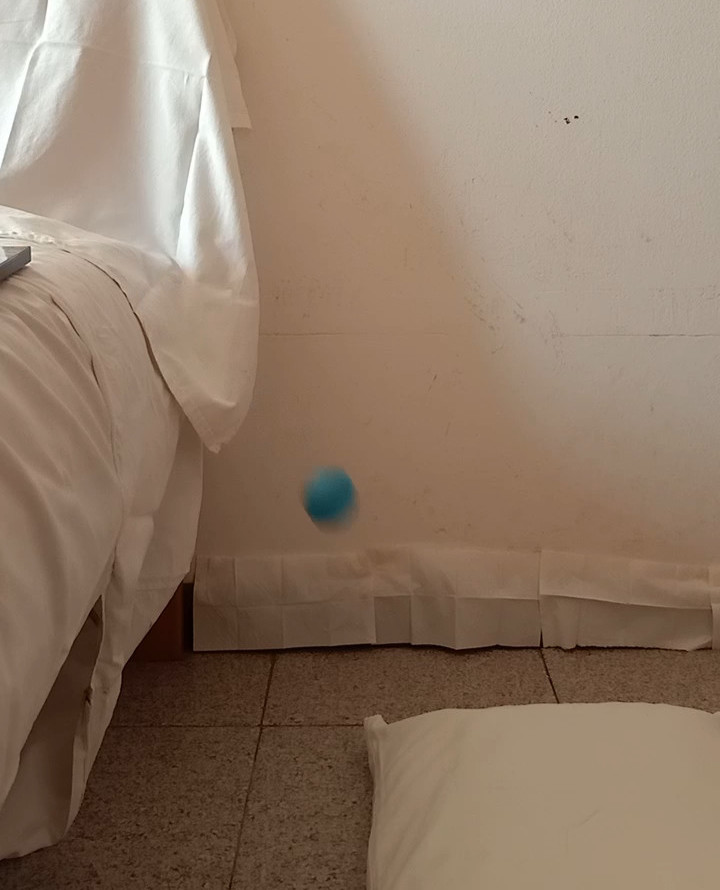
\includegraphics[width=\textwidth]{setup_proiettile}
  \caption{L'apparato sperimentale per studiare il moto di un proiettile.}
  \label{fig:setup_proiettile}
\end{figure}

\section{Gli elementi del gioco}
Il gioco di modellamento richiede prima di tutto la scelta
dei suoi componenti: tabellone e pedine.

\subsection{Il tabellone}
Il tabellone rappresenta in sistema di riferimento scelto per studiare
il sistema: nel nostro caso la coppia di assi cartesiani avente
origine nel punto in cui la pallina da ping-pong si stacca dal
piano orizzontale. L'asse $x$ è stato scelto parallelo al pavimento
con verso a destra e l'asse $y$ diretto come la forza gravitazionale
con verso in alto.

\subsection{Le pedine}
Le pedine rappresentano i corpi modellati come punti materiali
presenti nel sistema che stiamo studiando:

\begin{itemize}
\item La pallina da ping-pong di massa $m$;
\item Il pianeta Terra di massa $M \gg m$.
\end{itemize}

\section{Vincere il gioco}
Per vincere il gioco, dobbiamo produrre un modello valido
der il moto del proiettile. Per valutare la validità
del modello, ci proponiamo di prevedere la velocità iniziale
del proiettile dalla conoscenza della sua altezza iniziale
$h$ e della gittata $d$ raggiunta.

\section{Le mosse}
Possiamo compiere un certo numero di mosse, scelte tra il set
delle mosse valide, quello della dinamica newtoniana, per
condurre un gioco:

\begin{itemize}
\item Assegnare alle particelle posizioni e velocità iniziali nel sistema di riferimento scelto;
\item o interazioni consistenti con le leggi di interazione generali;
\item calcolare le traiettorie dalle leggi generali della dinamica;
\item validare il modello confrontandolo con il mondo fisico.
\end{itemize}

Tutte le precedenti sono mosse valide.

\bibliography{bibliografia}{}
\bibliographystyle{plain}

\end{document}
